\chapter{I$^2$C Configuration}
\label{chap:I2C}


In normal configuration the second I$^2$C-Bus of the Raspberry Pi is set up as two of the output pins of the DSI Display Connector resp. the CSI Camera Connector.\\
To make the setup of the quadrocopter as easy as possible and with respect to the weight and soldering/cabling these output pins were redirecteed to two of the 40 pins of the GPIO Header.\\

This gets done by useage of a Python-script (see below) which gets excecuted while booting the system. To get this configuration running two additional files need to be edited.\\\\
In "/boot/cmdline.txt"\\
\ttfamily bcm2708.vc\_i2c\_override=1 \\
\normalfont has to be added\\
in "/etc/modprobe.d/i2c\_o\_enable.conf"\\
\ttfamily{blacklist snd\_soc\_tas5713} \\
\normalfont has to be added.\\

After this the GPIO port 27 is configured as SDA0 and the GPIO port 28 as SCL0.

\begin{figure}[H]
	\centering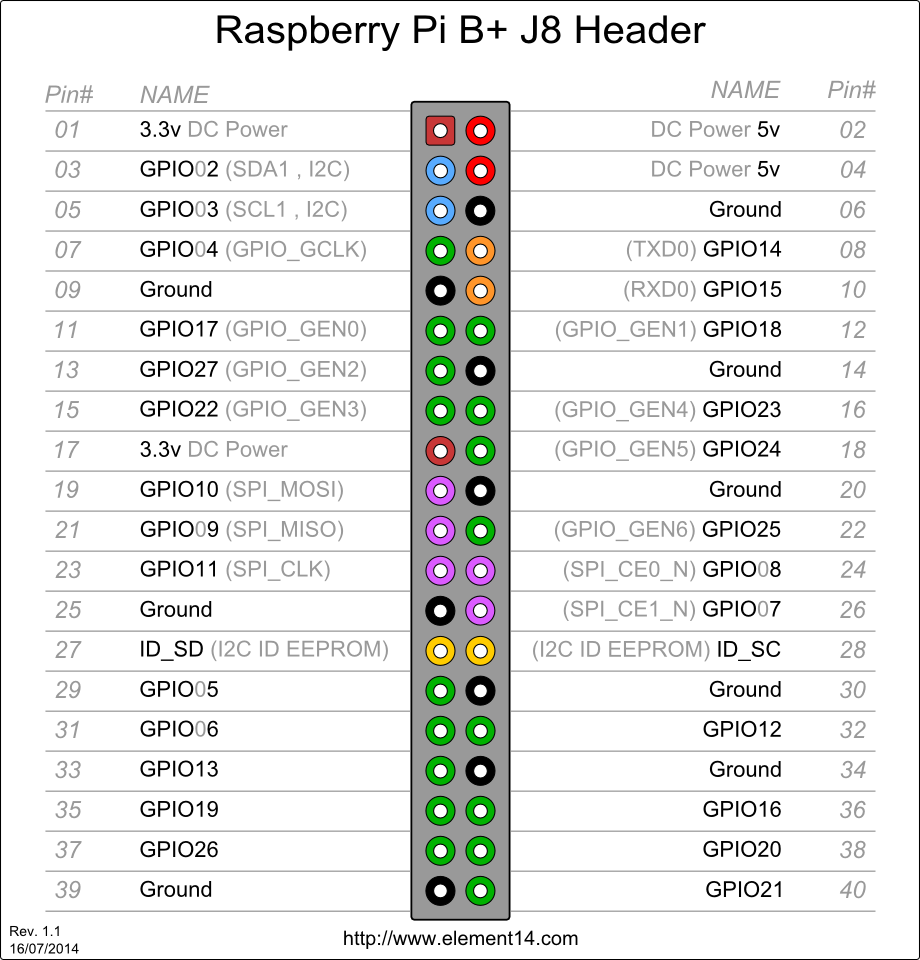
\includegraphics[width=0.5\textwidth]{fig/ch-i2c_configuration/gpios}
	\caption{GPIOs \footnotemark}
	\label{fig:gpios}
\end{figure}
\footnotetext{\url{http://www.element14.com/community/servlet/JiveServlet/previewBody/68203-102-6-294412/GPIO.png}}
\newpage


\lstinputlisting[language=Python, basicstyle=\tiny, caption=I$^2$C0 Port-Configuration]{add_files/I2C0_Config_OS.py}




